% Niveau :      PCSI *
% Discipline :  Chimie Orga
% Mots clés :   IR RMN

\begin{exercise}{Identification IR RMN 1}{1}{PCSI}
{Chimie organique I,Spectroscopie,RMN,Infrarouge}{bermu}

À l'aide des spectres IR et RMN $^{1}$H donnés ci-dessous, ainsi que des tables fournies en annexe, identifier la structure et attribuer les signaux spectroscopiques pertinents de ce composé de formule brute $\mathrm{C_{10}H_{14}O}$.
 
\vspace{2em}
 
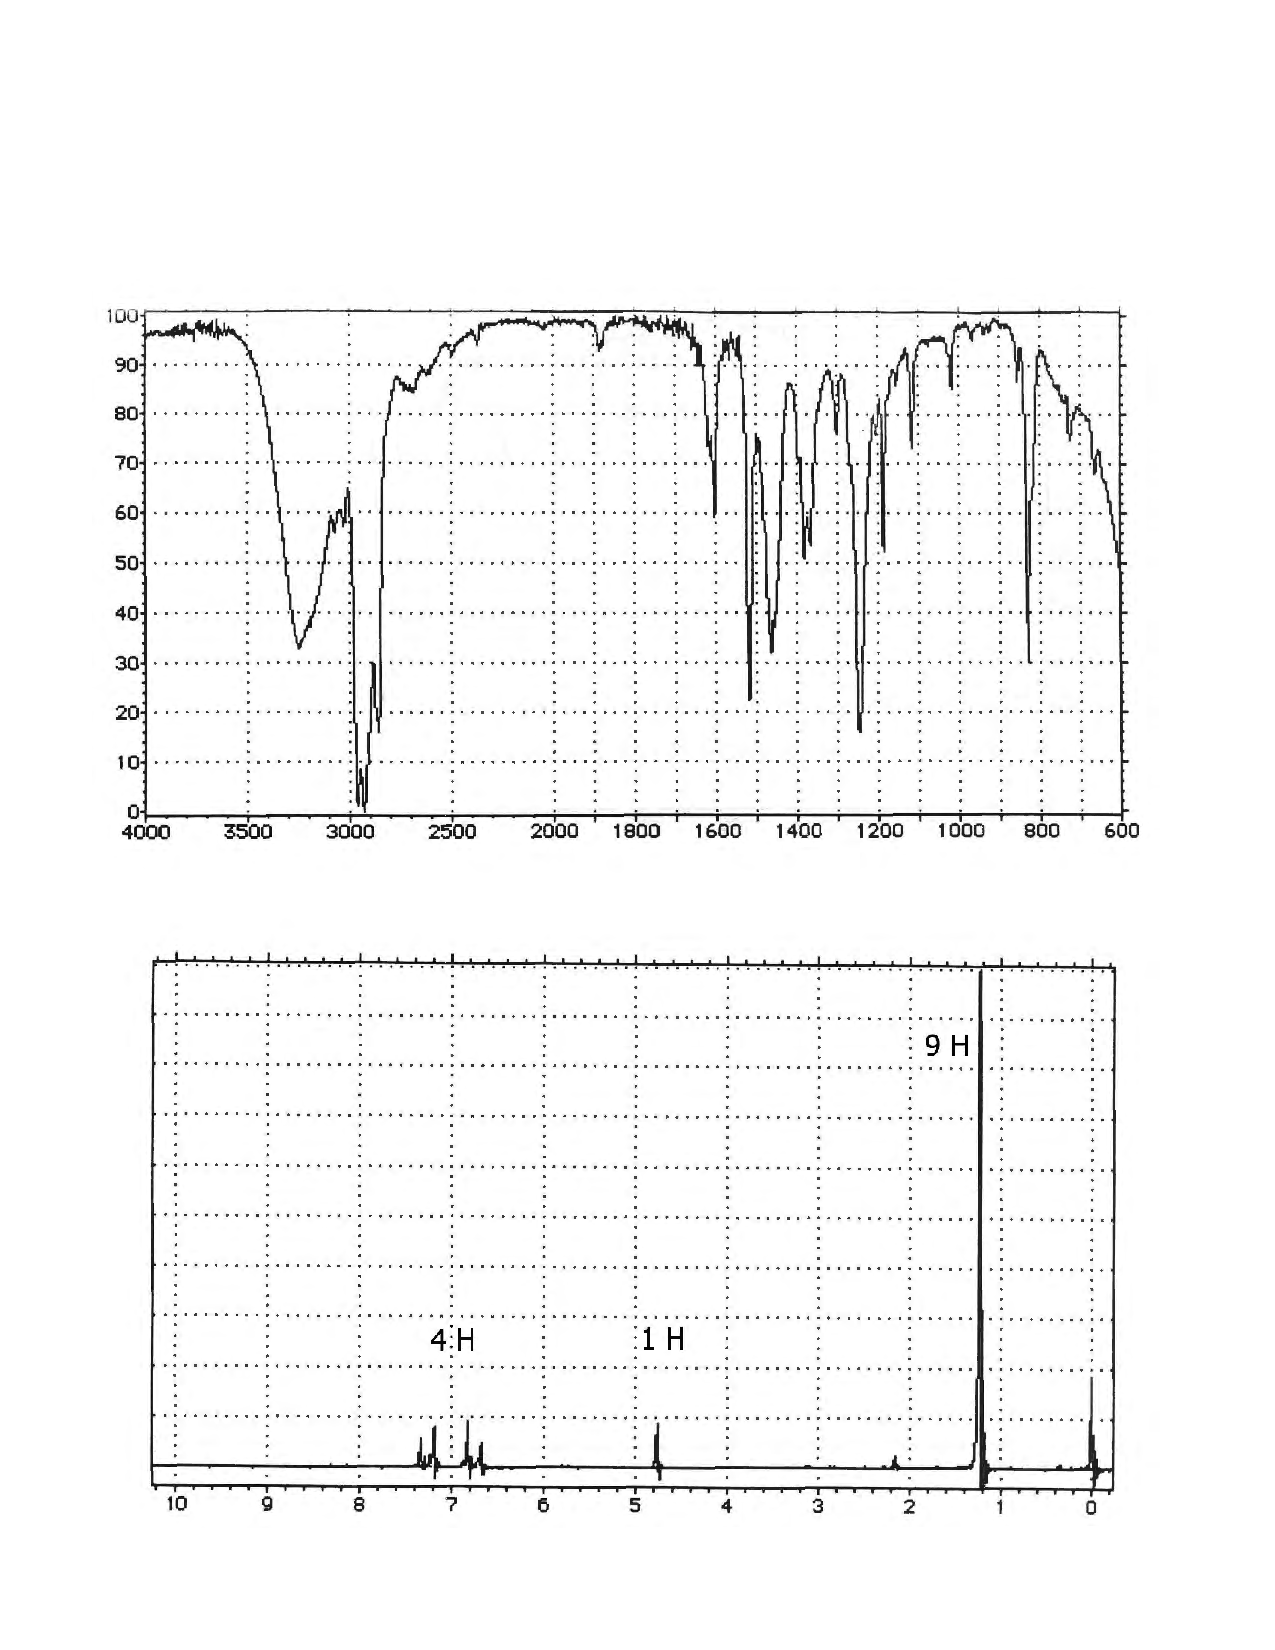
\includegraphics[width=\linewidth]{chimiePC/orga/IR_RMN_1.pdf}

\end{exercise}

\begin{solution}
\begin{center}
    \chemfig{HO-*6(=-=(-(-[:90]CH_3)(-CH_3)(-[:-90]CH_3))-=-)}
\end{center}
\end{solution}

\begin{exercise}{Identification IR RMN 2}{2}{PCSI}
{Chimie organique I,Spectroscopie,RMN,Infrarouge}{bermu}

À l'aide des spectres IR et RMN $^{1}$H donnés ci-dessous, ainsi que des tables fournies en annexe, identifier la structure et attribuer les signaux spectroscopiques pertinents de ce composé de formule brute $\mathrm{C_4H_{10}O_2}$.
 
\vspace{2em}
 
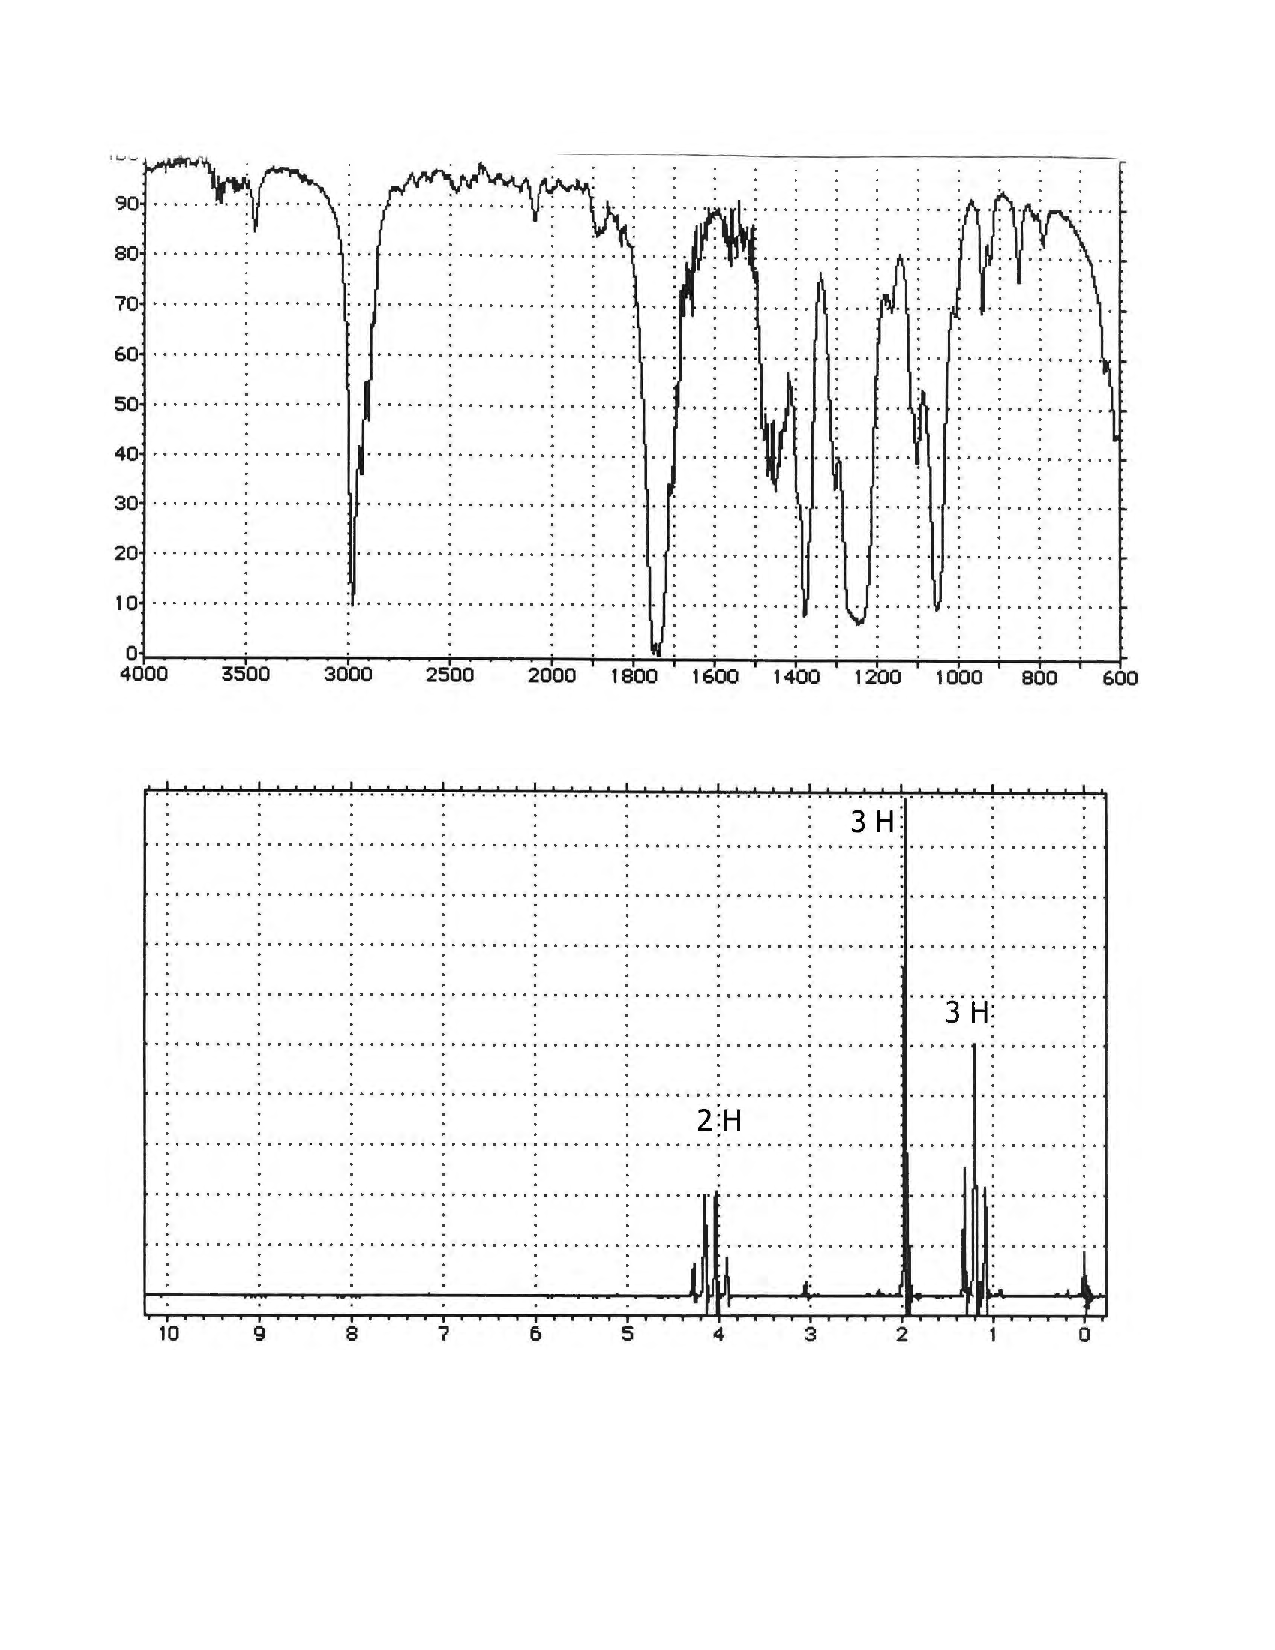
\includegraphics[width=\linewidth]{chimiePC/orga/IR_RMN_2.pdf}

\end{exercise}

\begin{solution}
\begin{center}
    \chemfig{-[1](=[3]O)-[-1]O-[1]-[-1]}
\end{center}
\end{solution}

\begin{exercise}{Identification IR RMN 3}{1}{PCSI}
{Chimie organique I,Spectroscopie,RMN,Infrarouge}{bermu}

À l'aide des spectres IR et RMN $^{1}$H donnés ci-dessous, ainsi que des tables fournies en annexe, identifier la structure et attribuer les signaux spectroscopiques pertinents de ce composé de formule brute $\mathrm{C_{10}H_{14}}$.
 
\vspace{2em}
 
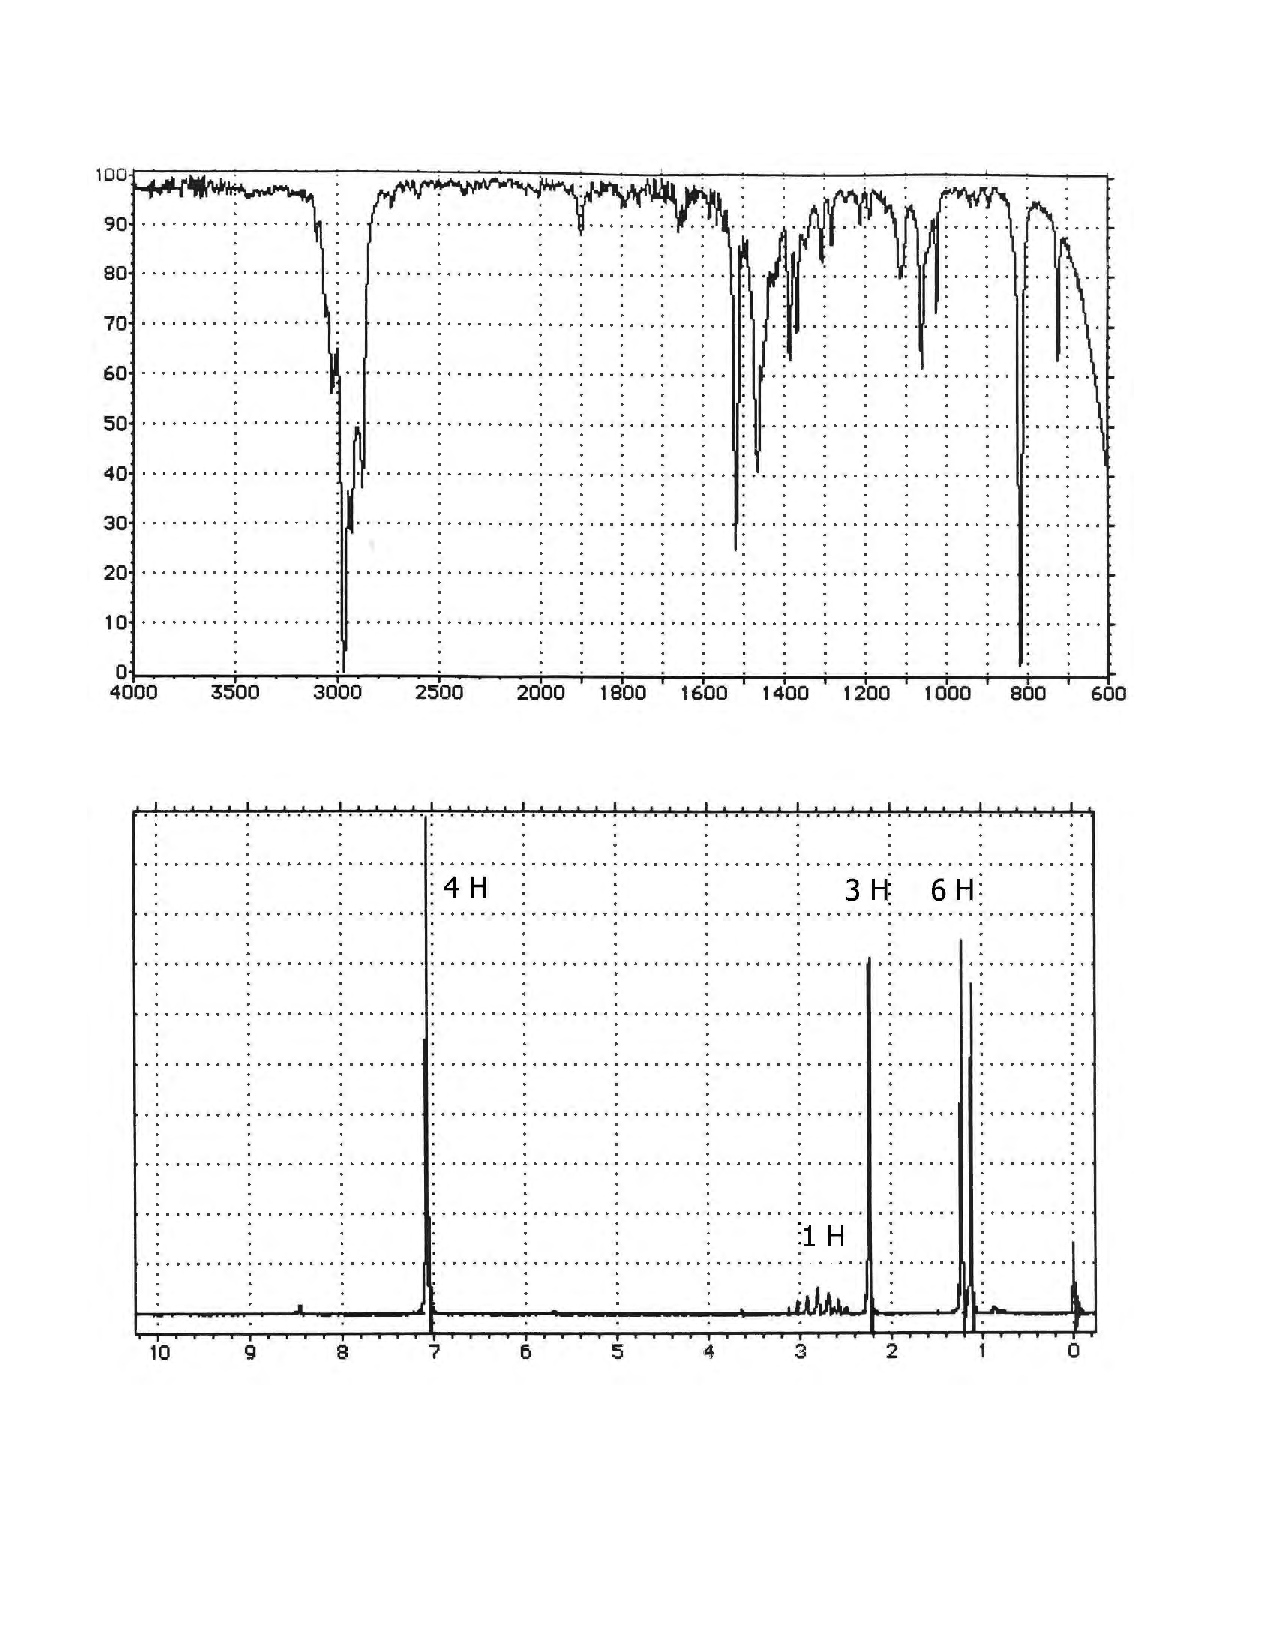
\includegraphics[width=\linewidth]{chimiePC/orga/IR_RMN_3.pdf}

\end{exercise}

\begin{solution}
\begin{center}
    \chemfig{H_3C-*6(=-=(-(-[2]CH_3)(-[-2]CH_3))-=-)}
\end{center}
\end{solution}

\begin{exercise}{Identification IR RMN 4}{2}{PCSI}
{Chimie organique I,Spectroscopie,RMN,Infrarouge}{bermu}

À l'aide des spectres IR et RMN $^{1}$H donnés ci-dessous, ainsi que des tables fournies en annexe, identifier la structure et attribuer les signaux spectroscopiques pertinents de ce composé de formule brute $\mathrm{C_9H_{10}O_2}$.
 
\vspace{2em}
 
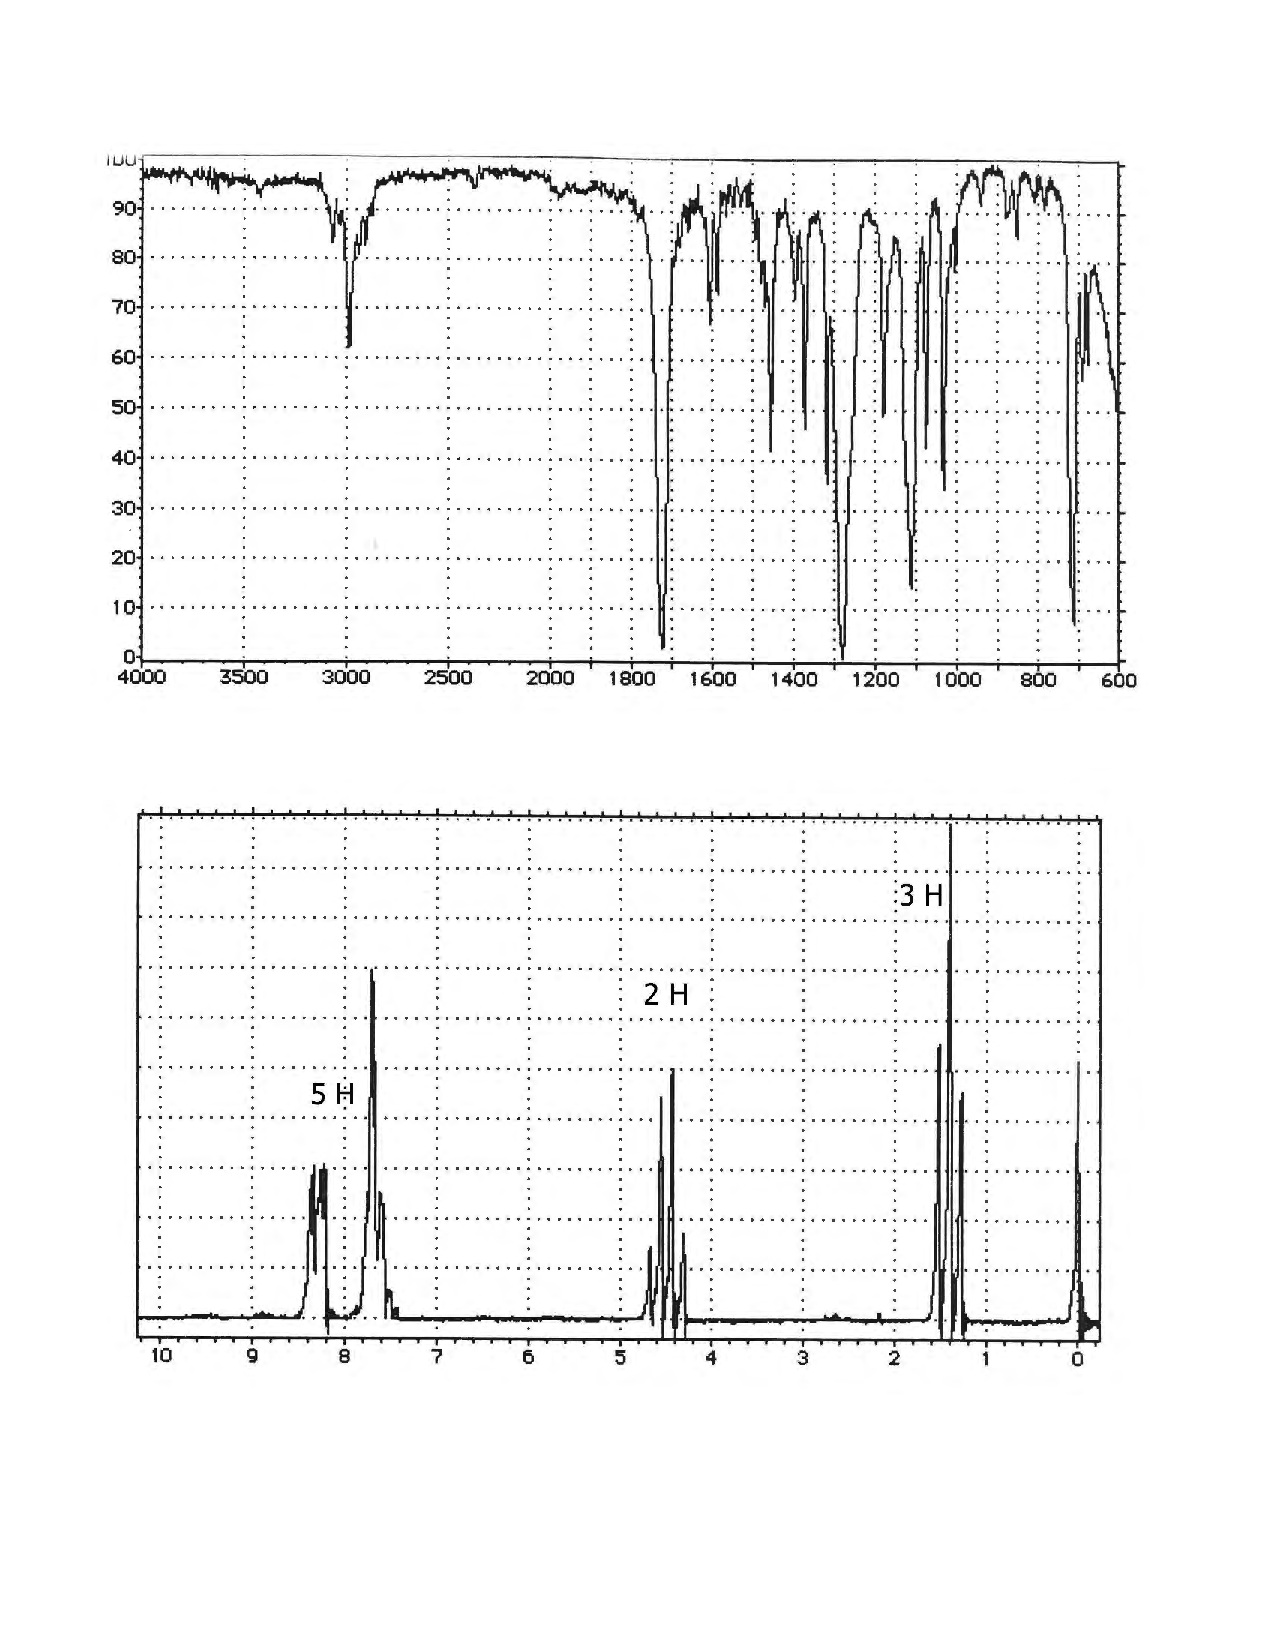
\includegraphics[width=\linewidth]{chimiePC/orga/IR_RMN_4.pdf}

\end{exercise}

\begin{solution}
\begin{center}
    \chemfig{[2]*6(=-(-[1](=[3]O)-[-1]O-[1]-[-1])=-=-)}
\end{center}
\end{solution}

\begin{exercise}{Identification IR RMN 5}{2}{PCSI}
{Chimie organique I,Spectroscopie,RMN,Infrarouge}{bermu}

À l'aide des spectres IR et RMN $^{1}$H donnés ci-dessous, ainsi que des tables fournies en annexe, identifier la structure et attribuer les signaux spectroscopiques pertinents de ce composé de formule brute $\mathrm{C_5H_{10}O_2}$.
 
\vspace{2em}
 
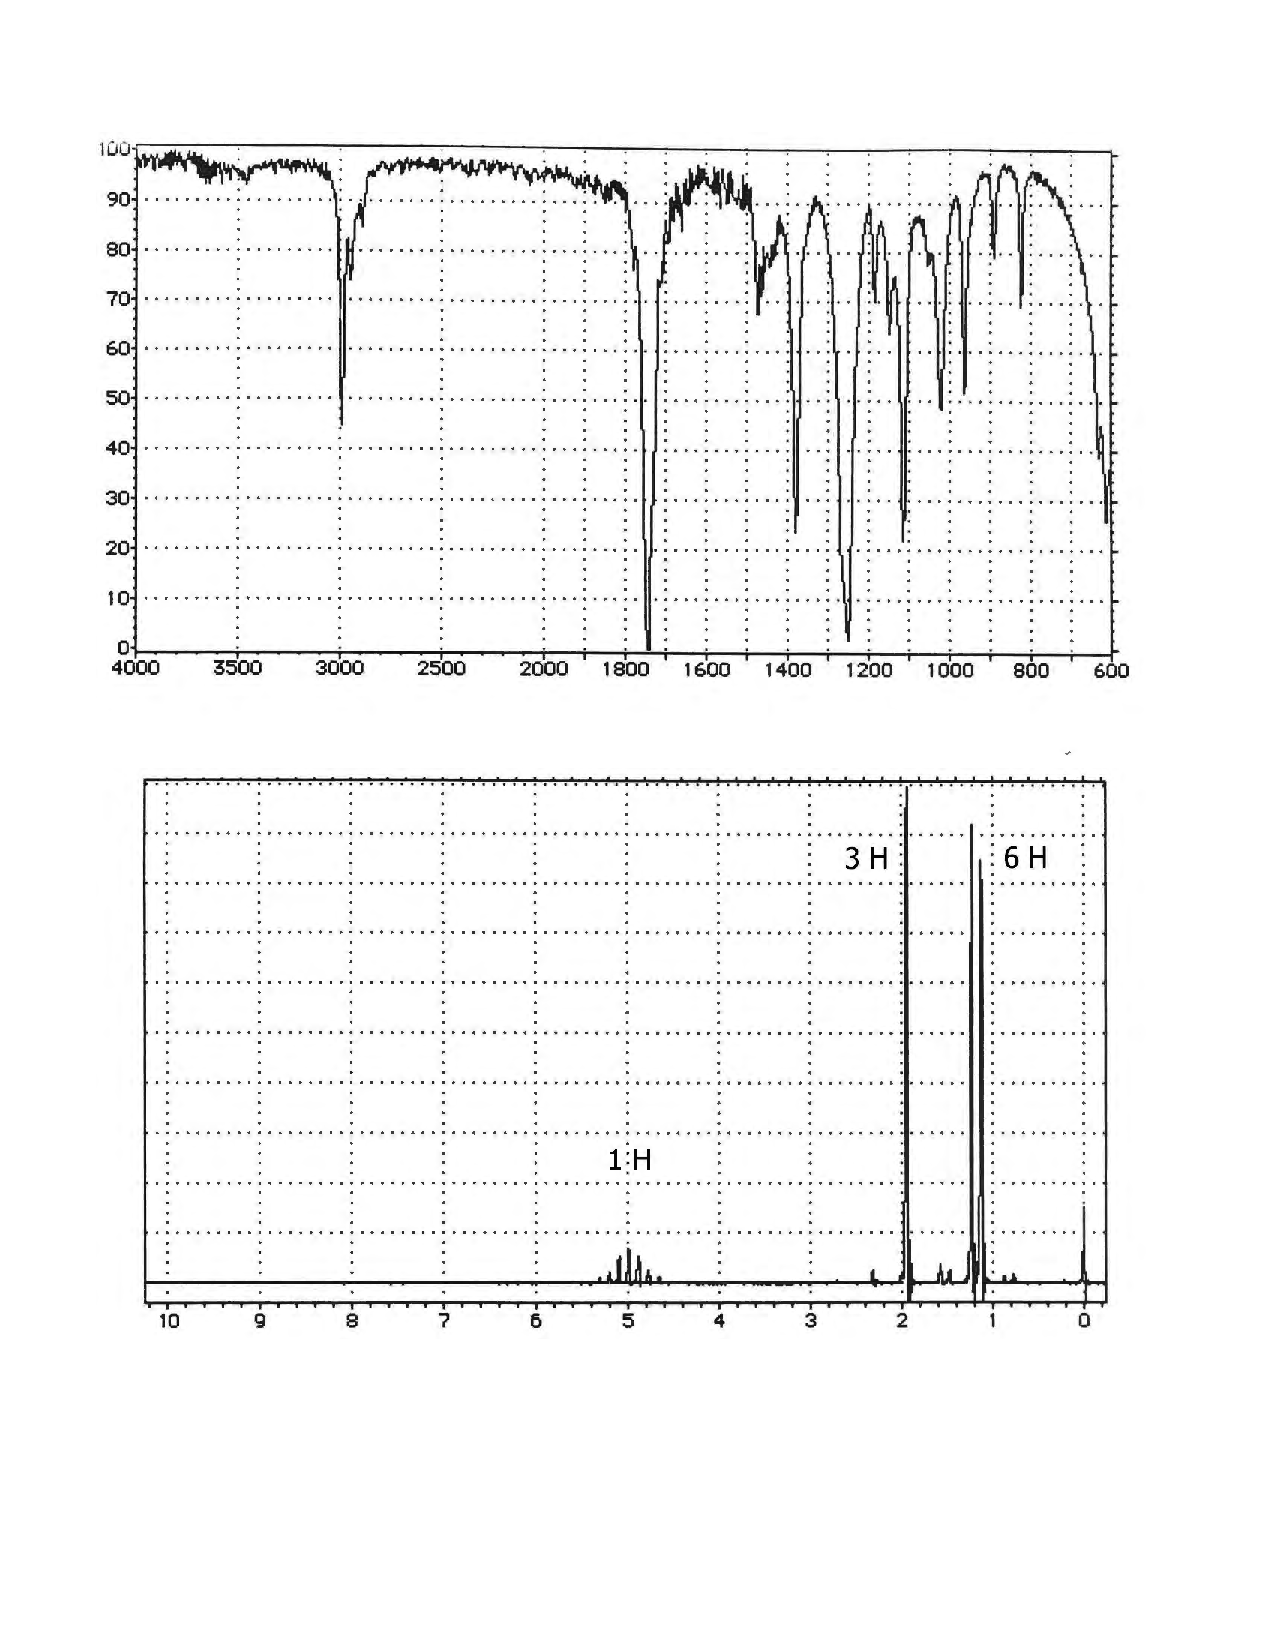
\includegraphics[width=\linewidth]{chimiePC/orga/IR_RMN_5.pdf}

\end{exercise}
\begin{solution}
\begin{center}
    \chemfig{-[1](=[3]O)-[-1]O-[1](-[3])-[-1]}
\end{center}
\end{solution}

\begin{exercise}{Identification IR RMN 6}{1}{PCSI}
{Chimie organique I,Spectroscopie,RMN,Infrarouge}{bermu}

À l'aide des spectres IR et RMN $^{1}$H donnés ci-dessous, ainsi que des tables fournies en annexe, identifier la structure et attribuer les signaux spectroscopiques pertinents de ce composé de formule brute $\mathrm{C_3H_6O_2}$.
 
\vspace{2em}
 
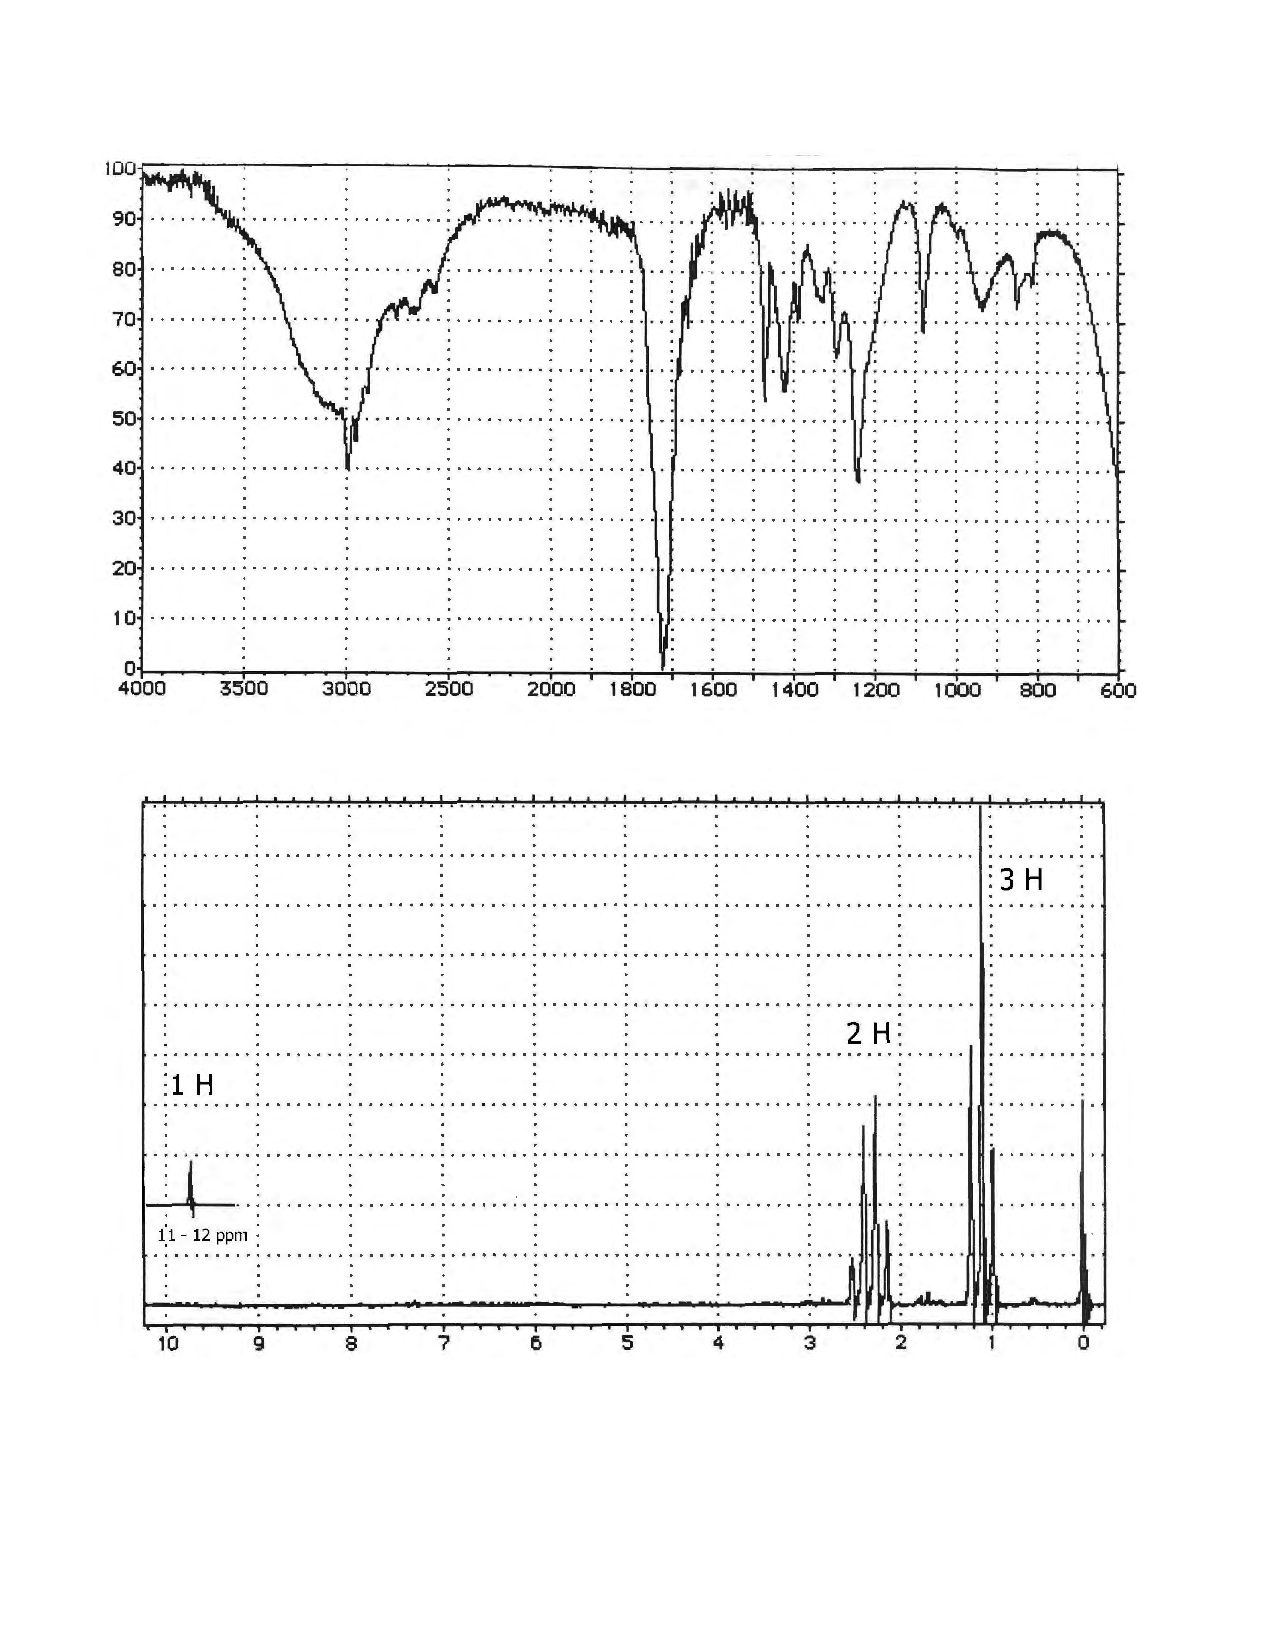
\includegraphics[width=\linewidth]{chimiePC/orga/IR_RMN_6.pdf}

\end{exercise}

\begin{solution}
\begin{center}
    \chemfig{-[-1]-[1](=[3]O)-[-1]OH}
\end{center}
\end{solution}

\begin{exercise}{Identification IR RMN 7}{2}{PCSI}
{Chimie organique I,Spectroscopie,RMN,Infrarouge}{bermu}

À l'aide des spectres IR et RMN $^{1}$H donnés ci-dessous, ainsi que des tables fournies en annexe, identifier la structure et attribuer les signaux spectroscopiques pertinents de ce composé de formule brute $\mathrm{C_9H_{21}N}$.
 
\vspace{2em}
 
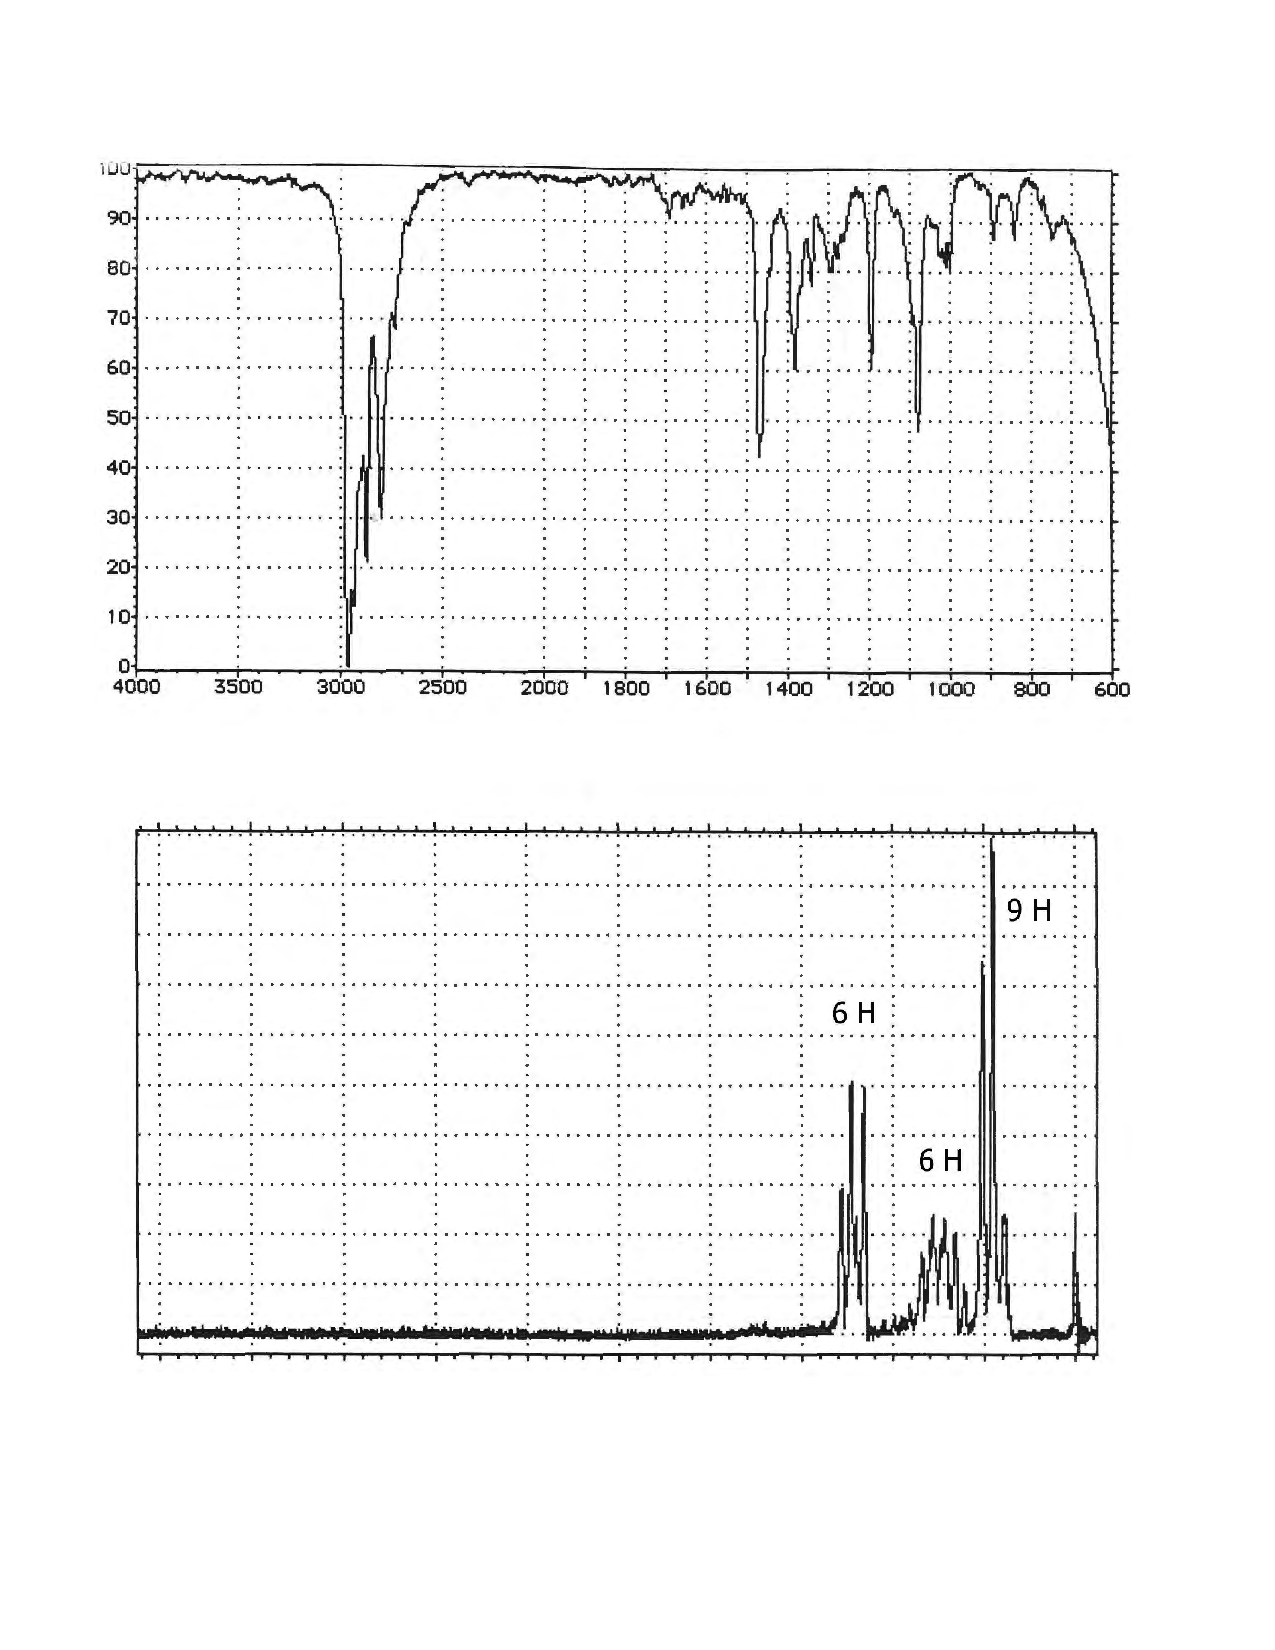
\includegraphics[width=\linewidth]{chimiePC/orga/IR_RMN_7.pdf}

\end{exercise}

\begin{solution}
\begin{center}
    \chemfig{N-[@{left,.5}1]-[-1]-[1]-[@{right,0.75}-1,,,,draw=none]}
    \polymerdelim[height = 5pt, indice = \!3]{left}{right}
\end{center}
\end{solution}

\begin{exercise}{Identification IR RMN 8}{2}{PCSI}
{Chimie organique I,Spectroscopie,RMN,Infrarouge}{bermu}

À l'aide des spectres IR et RMN $^{1}$H donnés ci-dessous, ainsi que des tables fournies en annexe, identifier la structure et attribuer les signaux spectroscopiques pertinents de ce composé de formule brute $\mathrm{C_5H_7NO_2}$.
 
\vspace{2em}
 
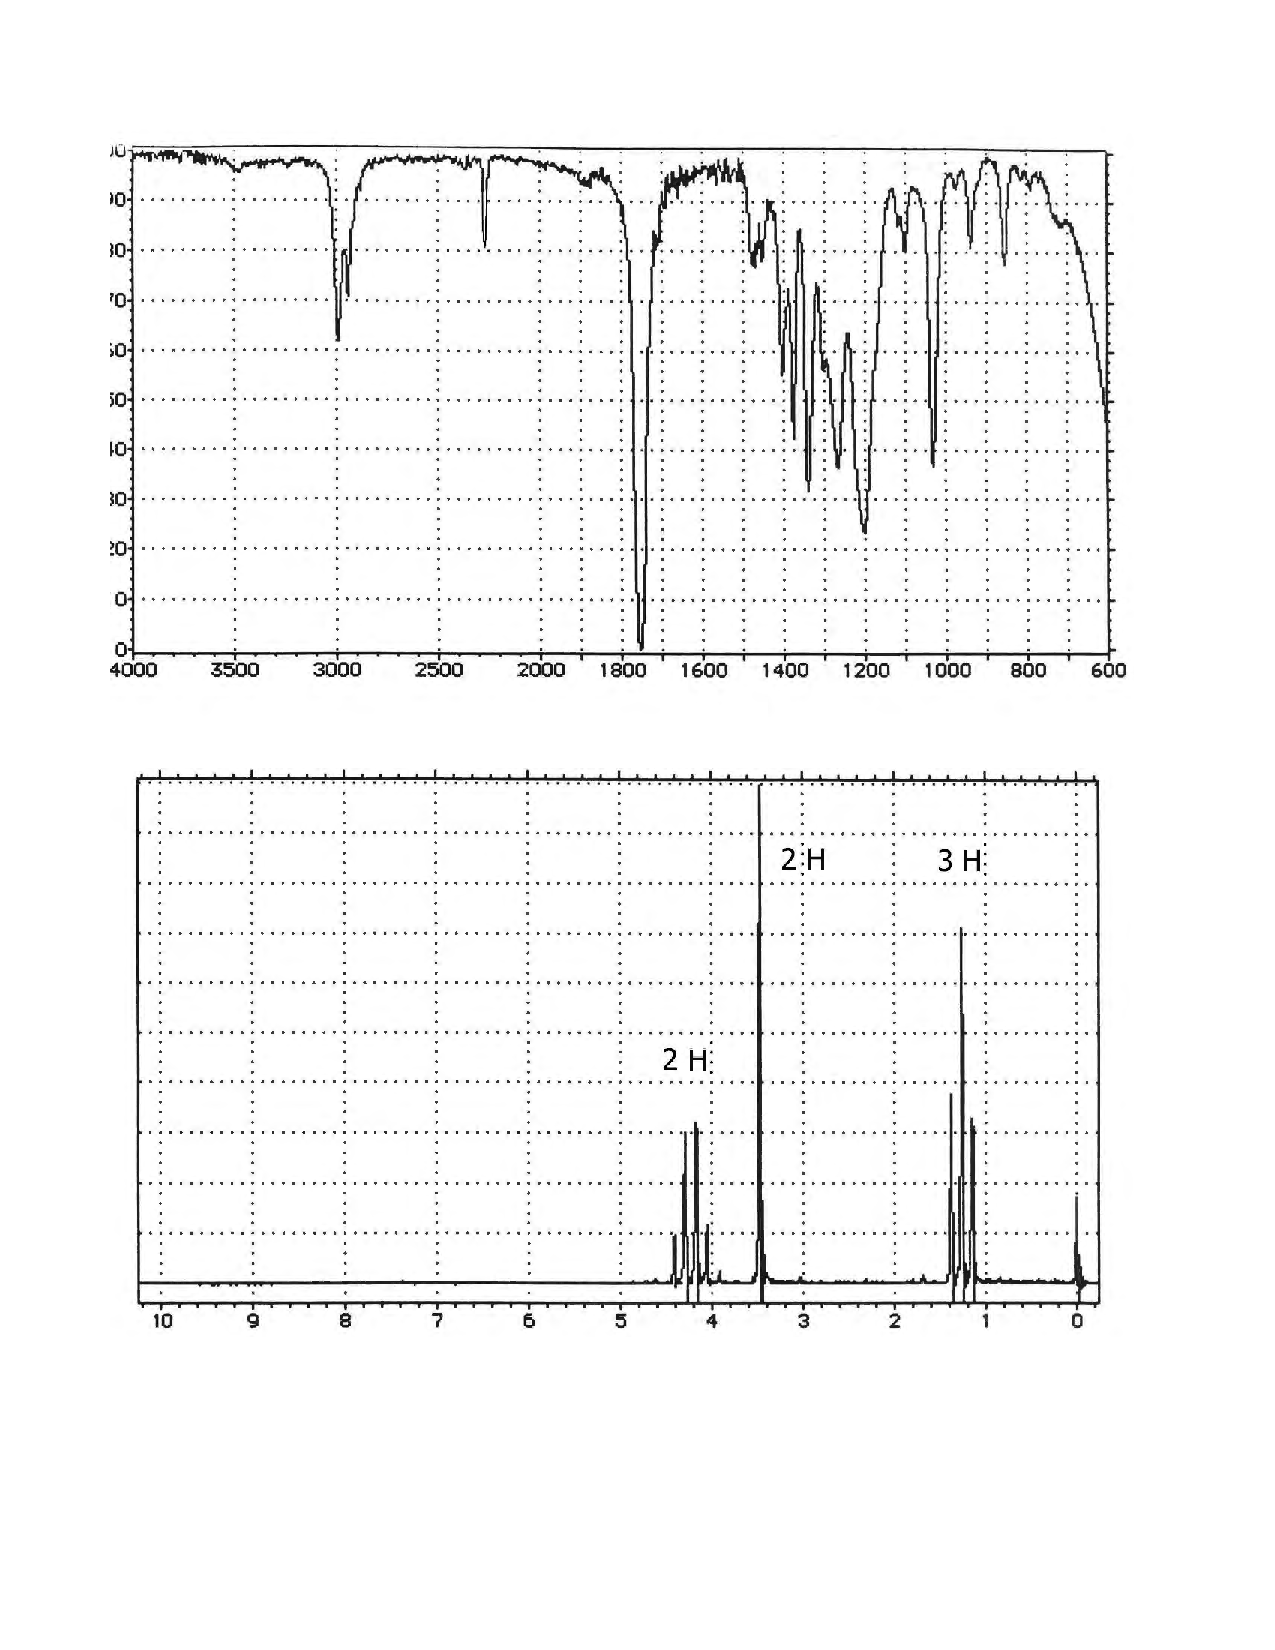
\includegraphics[width=\linewidth]{chimiePC/orga/IR_RMN_8.pdf}

\end{exercise}

\begin{solution}
\begin{center}
    \chemfig{-[-1]-[1](=[3]O)-[-1]O-[1]-[-1]~[-1]N}
\end{center}
\end{solution}